%%%%%%%%%%%%%%%%%%%%%%%%%%%%%%%%%%%%%%%%%%%%%%%%%%%%%%%%%%%%%%%%%%%%%%%%
%    INSTITUTE OF PHYSICS PUBLISHING                                   %
%                                                                      %
%   `Preparing an article for publication in an Institute of Physics   %
%    Publishing journal using LaTeX'                                   %
%                                                                      %
%    LaTeX source code `ioplau2e.tex' used to generate `author         %
%    guidelines', the documentation explaining and demonstrating use   %
%    of the Institute of Physics Publishing LaTeX preprint files       %
%    `iopart.cls, iopart12.clo and iopart10.clo'.                      %
%                                                                      %
%    `ioplau2e.tex' itself uses LaTeX with `iopart.cls'                %
%                                                                      %
%%%%%%%%%%%%%%%%%%%%%%%%%%%%%%%%%%
%
%
% First we have a character check
%
% ! exclamation mark    " double quote  
% # hash                ` opening quote (grave)
% & ampersand           ' closing quote (acute)
% $ dollar              % percent       
% ( open parenthesis    ) close paren.  
% - hyphen              = equals sign
% | vertical bar        ~ tilde         
% @ at sign             _ underscore
% { open curly brace    } close curly   
% [ open square         ] close square bracket
% + plus sign           ; semi-colon    
% * asterisk            : colon
% < open angle bracket  > close angle   
% , comma               . full stop
% ? question mark       / forward slash 
% \ backslash           ^ circumflex
%
% ABCDEFGHIJKLMNOPQRSTUVWXYZ 
% abcdefghijklmnopqrstuvwxyz 
% 1234567890
%
%%%%%%%%%%%%%%%%%%%%%%%%%%%%%%%%%%%%%%%%%%%%%%%%%%%%%%%%%%%%%%%%%%%
%
\documentclass[12pt, UK english]{iopart}
\newcommand{\gguide}{{\it Preparing graphics for IOP Publishing journals}}
%Uncomment next line if AMS fonts required
%\usepackage{iopams} 

\usepackage{hyperref}
\usepackage[space=true]{accsupp}
% requires the latest version of package accsupp
\newcommand{\copyablespace}{\BeginAccSupp{method=hex,unicode,ActualText=00A0}\ \EndAccSupp{}}


%%%%%%%%%%%%%%%%%%%%%%%%%%%%%%%%%%%%%%%%%%%%%%%%%%%%%%%%%%%%%%%%%%%
% Custom
%%%%%%%%%%%%%%%%%%%%%%%%%%%%%%%%%%%%%%%%%%%%%%%%%%%%%%%%%%%%%%%%%%%
\usepackage[T1]{fontenc}           % Embed fonts
\usepackage{textcomp,gensymb}      % \degree

\usepackage{polyglossia}                         % Define languages (Umlaute)
\setdefaultlanguage[variant=american]{english}   % Accent of main language
\setotherlanguage{german}                        % We also have german words
\usepackage[autostyle=true]{csquotes}            % Define quotation style
\MakeOuterQuote{"}                               % Text wrapped in "..." is recognized as a quotation

\usepackage{amssymb}                  % Math stuff
\usepackage{graphicx}                 % Import Pictures + PDFs
\usepackage[svgnames]{xcolor}         % Enabling colors by their 'svgnames'
\usepackage{listings}                 % Code listings  See: https://en.wikibooks.org/wiki/LaTeX/Source_Code_Listings

\usepackage{subcaption} % subfigures
\usepackage{caption}    % itemize in caption

%%%%%%%%%%%%%%%%%%%%%%%%%%%%%%%%%%%%%%%%%%%%%%%%%%%%%%%%%%%%%%%%%%%
% Definitions
%%%%%%%%%%%%%%%%%%%%%%%%%%%%%%%%%%%%%%%%%%%%%%%%%%%%%%%%%%%%%%%%%%%
\definecolor{fzjblue}{HTML}{005B81}
\definecolor{light-gray}{gray}{0.97}
\definecolor{semilight-gray}{gray}{0.67}
\definecolor{mygreen}{rgb}{0,0.6,0}

% Custom code listings environment
\lstset{
  language=Python,
  backgroundcolor=\color{light-gray},   % choose the background color; you must add \usepackage{color} or \usepackage{xcolor}
  basicstyle=\linespread{1}\footnotesize\ttfamily,        % the size of the fonts that are used for the code
  commentstyle=\color{mygreen},
  frame=single,
  keywordstyle=\color{blue},       % keyword style
  tabsize=4,	                   % sets default tabsize to 2 spaces
  showtabs=false,
  rulecolor=\color{black},
  columns=fullflexible,
  literate={\ }{{\copyablespace}}1
}

\usepackage[prependcaption, textsize=tiny]{todonotes}

%%%%%%%%%%%%%%%%%%%%%%%%%%%%%%%%%%%%%%%%%%%%%%%%%%%%%%%%%%%%%%%%%%%
% Commands
%%%%%%%%%%%%%%%%%%%%%%%%%%%%%%%%%%%%%%%%%%%%%%%%%%%%%%%%%%%%%%%%%%%
\newcommand{\python}[0]{\texttt{Python}}
\newcommand{\vpython}[0]{\texttt{VPython}}
\newcommand{\abs}[1]{\left\vert #1 \right\vert}
\newcommand{\code}[1]{{\scriptsize\colorbox{light-gray}{\texttt{#1}}}}


%%%%%%%%%%%%%%%%%%%%%%%%%%%%%%%%%%%%%%%%%%%%%%%%%%%%%%%%%%%%%%%%%%%
% Here it starts
%%%%%%%%%%%%%%%%%%%%%%%%%%%%%%%%%%%%%%%%%%%%%%%%%%%%%%%%%%%%%%%%%%%
\begin{document}

\title[A primer to numerical simulations]{A primer to numerical simulations: The perihelion motion of Mercury}

\author{I. Hammer, C. Hanhart, C. Körber and C. Müller}

\address{Forschungszentrum Jülich}
\ead{c.hanhart@fz-juelich.de}
\vspace{10pt}
%\begin{indented}
%\item[]February 2014
%\end{indented}

\begin{abstract}
Numerical simulations are playing an increasingly important role in modern science.
In this work it is suggested to use a numerical study of the famous perihelion motion of the planet Mercury (one of the prime observables supporting Einsteins General Relativity) as a test case to teach numerical simulations to high school students.
The paper includes details about the development of the code as well as a discussion of the visualization of the results.
In addition a method is discussed how to estimate the size of the effect a priori. 
\end{abstract}

% Uncomment for PACS numbers
%\pacs{00.00, 20.00, 42.10}
%
% Uncomment for keywords
%\vspace{2pc}
%\noindent{\it Keywords}: XXXXXX, YYYYYYYY, ZZZZZZZZZ
%
% Uncomment for Submitted to journal title message
%\submitto{\JPA}
%
% Uncomment if a separate title page is required
%\maketitle
% 
% For two-column output uncomment the next line and choose [10pt] rather than [12pt] in the \documentclass declaration
%\ioptwocol
%

\listoftodos

%%%%%%%%%%%%%%%%%%%%%%%%%%%%%%%%%%%%%%%%%%%%%%%%%%%%%%%%%%%%%%%%%%%
\section{Introduction}\label{sec:intro}
%%%%%%%%%%%%%%%%%%%%%%%%%%%%%%%%%%%%%%%%%%%%%%%%%%%%%%%%%%%%%%%%%%%

Numerical simulations play a key role in modern physics for they allow one to tackle theoretical problems not accessible otherwise, e.g., since there are too many particle participating in the system (as in simulations for weather predictions) or the interactions are too complicated to allow for a systematic, perturbative approach (as in theoretical descriptions of nuclear particles at the fundamental level).
This paper introduces a project that can be used to demonstrate the power of numerical simulations.
On the example of the perihelion motion of the planet Mercury the students are supposed to get in touch with
\begin{itemize}
\item the importance of differential equations in theoretical physics;
\item the numerical implementation of Newtonian dynamics;
\item systematic tests and optimization of computer codes;
\item effective tools to estimate the result a priori as an important cross check;
\item the visualization of numerical results using \texttt{VPython}.
\end{itemize}
The course as well as this paper is structured as follows: after an introduction to Newtonian dynamics and the concepts of differential equations, their discretization is discussed based on Newtons law of gravitation and possible extensions thereof.
Afterwards the visualization of the resulting trajectories using \texttt{VPython} is introduced and applied to the problem at hand. In particular tools are developed to extract the relevant quantity from the result of the simulation.
Finally the principle of dimensional analysis is presented as a tool to cross check, if the results of the simulation are sensible.

We are convinced that in order to excite the students for numerical simulations it is compulsory to demonstrate their power on an example that catches their interest.
This purpose is served perfectly by the case chosen here, since Einsteins equations of General Relativity are fascinating to a very broad public.
While their detailed study needs deeper knowledge in Differential Geometry, for the study outlined here very little math is necessary, such that high school students from about 10$^{\rm th}$ grade up should benefit from it.
This was already demonstrated in the "Schülderakademie Teilchenphysik", where an early version of this course was tested successfully on a group of 17 German high school students from 10$^{\rm th}$ to 13$^{\rm th}$ grade.



%%%%%%%%%%%%%%%%%%%%%%%%%%%%%%%%%%%%%%%%%%%%%%%%%%%%%%%%%%%%%%%%%%%
\section{Trajectories, velocities, accelerations and Newtons second law}\label{sec:tva}
%%%%%%%%%%%%%%%%%%%%%%%%%%%%%%%%%%%%%%%%%%%%%%%%%%%%%%%%%%%%%%%%%%%

We can say that we understand a physical system, if we can demonstrate that the assumed force leads to the trajectories observed.
In other words, we need to show that we can calculate the location in space of the object of interest at any point in time, once the initial conditions are fixed properly.
If we can neglect the finite size of this object (and in particular its orientation in space) the location is parametrized by a single three vector $\vec r(t)$.
As will become clear below, in order to describe and control the dynamics of a physical object in addition we need to be able to calculate its velocity, $\vec v(t)$, related to the location via
\begin{equation}\label{eq:x_update}
\vec r(t+\Delta t) = \vec r(t) + \vec v(t) \Delta t + ... \ , \label{eq:vdef}
\end{equation}
for some infinitesimally small $\Delta t$ and the acceleration, $\vec a(t)$ that describes the change of the velocity
\begin{eqnarray}\label{eq:v_update}
\vec v(t+\Delta t) = \vec v(t) + \vec a(t) \Delta t + ...\ . \label{eq:adef}
\end{eqnarray}
The dots in the above expressions indicate that there are in general additional terms that may be expressed with higher powers in $\Delta t$, however, for sufficiently small $\Delta t$ those can be safely neglected.
Thus we may define the time derivative via
\begin{equation}
\vec v(t) = \lim_{\Delta t\to 0} \frac{\Delta \vec r(t)}{\Delta t} =: \frac{d\vec r(t)}{d t}  = \dot{\vec  r}(t) \ ,
\end{equation}
where $\Delta \vec r(t)=\vec r(t+\Delta t)-\vec r(t)$ and we introduced with the last expression a common short hand notation for time derivatives.
Analogously we get
\begin{eqnarray}
\vec a(t) &=& \lim_{\Delta t\to 0} \frac{\Delta \vec v(t)}{\Delta t} =: \frac{d\vec v(t)}{dt}  = \dot{\vec v}(t) \ , \\
 &=& \frac{d^2\vec r(t)}{dt^2}  = \ddot{\vec r}(t) \ ,
\end{eqnarray}
where we introduced in the second line the second derivative.

It was Newton who observed that if a body is at rest it will remain at rest, and if it is in motion it will remain in motion in a constant velocity in a straight line, unless it is acted upon by some force --- this is known as Newtons first law.
Said differently: a force $\vec F$ shows up by changing the motion of some object.
This is quantified in Newton's second law
\begin{equation}
\vec F(\vec r, t) = \frac{d}{dt}(m \vec v) \ .
\end{equation} 
If the mass does not change~\footnote{%
	A well known example where $m$ does change with time is a rocket, whose mass decreases as the rocket rises.
} with time, this reduces to the well known
\begin{equation}
\vec F(\vec r) = m \vec a(t) = m\dot{\vec v}(t) = m\ddot{\vec{r}}(t) \ . \label{eq:newton2}
\end{equation} 
Note that in general the force could depend also on the time or the velocity.
We here restrict ourselves to the case relevant for our example, where the force depends on the location only. 
Therefore, as soon as the force $\vec F(\vec r)$ is known for all $\vec r$ one can in principle calculate the trajectory, e.g., solving Eq.~(\ref{eq:newton2}) for $\vec r(t)$.
Sometimes this requires some advanced knowledge in math, sometimes no closed form solution exists.
However, alternatively one can calculate the whole trajectory of some test body that experiences this force by a successive application of the rules given in eqs.~(\ref{eq:vdef}) and (\ref{eq:adef}):
\begin{enumerate}
\item For a given time $t$, where $\vec r(t)$ and $\vec v(t)$ are known, use Eq.~(\ref{eq:newton2}) to calculate $\vec a(t)$.
\item Use Eq.~(\ref{eq:vdef}) to calculate $\vec r(t+\Delta t)$ and
\item then use Eq.~(\ref{eq:adef}) to calculate $\vec v(t+\Delta t)$.
\item Go back to (i) with $t\to t+\Delta t$.
\end{enumerate}
Clearly to initiate the procedure at some time $t_0$ both $\vec r(t_0)$ as well as $\vec v(t_0)$ must be known --- the  trajectories depend on these initial conditions~\footnote{%
	In general a differential equation of $n^{\rm th}$ degree (where the highest derivative is $n$) needs $n$ initial conditions specified.
	For $n=2$ those are often chosen as location and velocity at some defined time, but one may as well pick two location at different times.%
}.

For this procedure to work $\Delta t$ must be sufficiently small.
What this means depends on the process studied.
One way to estimate, if $\Delta t$ is small enough, is to verify, if the relation
\begin{equation}
|\vec v(t)| \gg \frac12|\vec a(t)|\Delta t = \frac{1}{2m} |\vec F(\vec r(t)) |\Delta t\ . 
\label{eq:check}
\end{equation}
holds, since the next term neglected in Eq.~(\ref{eq:vdef}) reads $(1/2)a(t)(\Delta t)^2$.
Eq.~({\ref{eq:check}}) also shows that small (large) time steps are necessary (sufficient), if the force is strong (weak), since the time steps need to be small enough that all changes induced by the force get resolved.
Clearly, a relation as Eq.~({\ref{eq:check}}) can only provide guidance and can not replace a careful numerical check of the solutions: A valid result has to be insensitive the concrete value $\Delta t$ chosen --- in particular replacing $\Delta t$ by $\Delta t/2$ should not change the result significantly.



%%%%%%%%%%%%%%%%%%%%%%%%%%%%%%%%%%%%%%%%%%%%%%%%%%%%%%%%%%%%%%%%%%%
\section{Example: General Relativity and the perihelion motion of Mercury}\label{sec:gr}
%%%%%%%%%%%%%%%%%%%%%%%%%%%%%%%%%%%%%%%%%%%%%%%%%%%%%%%%%%%%%%%%%%%
For this concrete example the starting point for the force is Newtons law of gravitation
\begin{equation}
\vec F_N(\vec r) = - \frac{G_N m M_\odot}{r^2} \frac{\vec r}{r}\ ,
\end{equation}
where $G_N=6.67\times 10^{-11}$ m$^3$kg$^{-1}$s$^{-2}$ is the Newtonian constant of gravitation, $m$ is the mass of Mercury and $M_\odot=2\times 10^{30}$ kg is the mass of the sun.
In addition $r=|\vec r(t)|$ denotes the distance between sun and Mercury, when we assume that the sun is infinitely more heavy than the planet and located at the center of the coordinate system. 
Although this is not exact, since $m/M_\odot\sim 10^{-8}$ this is a pretty good approximation.
For later convenience we introduce the Schwarzschildradius of the sun
\begin{equation}
r_S=\frac{2G_N  M_\odot}{c^2} = 3 \ \mbox{km} \ ,
\end{equation}
where $c=3\times 10^8$ m/s denotes the speed of light.
Note that $r_S$ is the characteristic length scale of the gravitational field of the sun for --- up to the prefactor --- one can not form another quantity with dimensions of a length from $G_N$, $M_\odot$ and $c$.
This is what we need $r_S$ for later in the discussion.
That the Schwarzschild radius is also an important quantity to characterize black holes is not relevant for the discussion at hand.
With this Newtons second law reads 
\begin{equation}
	\ddot{r}      = - \frac{c^2}{2}\left(\frac{r_S}{r^2}\right) \, , \qquad
	\ddot{\vec r} =   \ddot{r} \, \frac{\vec{r}}{r} \, .
\label{eq:newton}
\end{equation}
In general an attractive force that vanishes at large distances leads,  depending on the initial conditions, either to bounded orbits or to open orbits --- in the latter case the planet simply disappears from the sun.
Depending on time available for the course it might be helpful to explain to the students the origin of this, however, since the most transparent reasoning needs an integration as well as the concept of angular momentum not necessarily familiar to the whole class, it appears in general more appropriate to work out together with the students that a moving body can not be kept by a force if its momentum is too large.
Then they may try to find closed orbits in the simulation, e.g., by varying the start velocity while keeping the start location fixed.

The bounded orbits that emerge from a potential that scales as $1/r$ are elliptic and fixed in space.
In particular the point of closest approach of the planet to the sun, the perihelion, does not move.
However, as soon as the potential deviates from $1/r$, the perihelion moves.
Because of this, the behavior of the perihelion is a very sensitive probe of the gravitational potential. 

The observed perihelion motion of Mercury is nowadays determined as $(574.10\pm 0.65)''$ per
100 earth years~\footnote{The symbol $''$ denotes "arc seconds": 1$''=(1/3600)^o$. }, but it should be noted that the bulk of this number
can be understood by the presence of other planets within the Newtonian theory, since
their gravitational force also acts on Mercury. However, a
residual motion of $\delta \Theta_M = (43)''$ in 100 earth years remained unexplained, until Einstein quantified the
predictions of General Relativity to this particular observable. \todo{@CH:citation here}

We allow for a movement of the perihelion by modifying the potential of Eq.~(\ref{eq:newton}) with the following ansatz
\begin{equation}
\ddot{\vec r} = - \frac{c^2}{2}\left(\frac{r_S}{r^2}\right)\left(1+\alpha\frac{r_S}{r}\right) \, \frac{\vec{r}}{r} \ ,
\label{eq:newton_art}
\end{equation}
where $\alpha$ is some parameter related to the effects by General Relativity.
The idea is that the correction must be dimension-less and should scale with some inverse power of $r$, for we still need to demand that the potential vanishes at large distances.
Since the only parameter of the system with dimension of a length is $r_S$, the correction should scale as $(r_S/r)$.
Replacing $r$ by a typical distance of Mercury to the sun, $(r_S/r_{MS})\sim 10^{-7}$, suggests that it should be sufficient to include this kind of term to first order only.\footnote{Considering another order would lead qualitatively to the same result, since every change in the potential leads to a perihelion motion. Only the value of the pre-factor would change.}
For comparison: the typical distance of the Venus, the neighbor of Mercury, to the sun is $(r_S/r_{VS}) \sim 5 \cdot 10^{-8}$.
Therefore the expected ratio of residual motion, favoring in the orbit period $T$, would result in
\begin{equation}
	\delta \Theta_V \approx \frac{1}{T_V} \delta \Theta_M T_M \frac{r_{MS}}{r_{VS}} \approx 9'' \, ,
\end{equation}
where $T_V$ ($T_M$) denotes the length of a venus (mercury) year. This precisely describes the experimental value of $9''$.



%%%%%%%%%%%%%%%%%%%%%%%%%%%%%%%%%%%%%%%%%%%%%%%%%%%%%%%%%%%%%%%%%%%
\section{Numerical Implementation}\label{sec:Numerical Implementation}
%%%%%%%%%%%%%%%%%%%%%%%%%%%%%%%%%%%%%%%%%%%%%%%%%%%%%%%%%%%%%%%%%%%

%------------------------------------------
\subsection{Describing the Motion with Python}
%------------------------------------------

In this section we present the numerical implementation as well as the visualisation of planetary trajectories and in
particular
the perihelion motion of Mercury.  We select \python{} (\url{https://www.python.org}) as  programming language, because \python{} is easy to learn, intuitive to understand and an open source language.
No prior knowledge of \python{} or any other programming language is required, as we explain all the necessary steps to create the simulation.
In appendix \ref{appendix:python} we give instructions for setting up \python{} on different operating systems.
We also provide a working example program that can be used as a template \url{this-upload-url}\todo{@arXiv: online link}.

To start the simulation one needs the "initial" distances and velocities, which are needed as input to the equation of motion [Eq.~(\ref{eq:x_update}) and Eq.~(\ref{eq:v_update})].
As described above, here  one can simplify the problem by placing one planet (the "infinitely" heavy sun) in the center of the coordinate system and describe the motion of the other planet (mercury) in a two-dimensional plane.  

Because the problem does not depend on the initial position of mercury on its orbit around the sun, we extract the parameters at the perihelion with $ \abs{\vec r_{MS}(0)} = 46 \cdot 10^6$km and $ \abs{\vec v_M(0)} = 59$km/s\footnote{\url{https://nssdc.gsfc.nasa.gov/planetary/factsheet/mercuryfact.html}}.
Since the computer does not understand physical units, one has to express each variable in an appropriate unit.
Both, for the numerical treatment and the intuitive understanding, it is useful to select parameters in a "natural range".
A useful choice for this problem is given e.g. by expressing distances in $R_0 = 10^{10}$ m and time intervals in days, $T_0 = 1$d, where $d$ refers to earth days, such that one mercury year is given by $T_M=88\,T_0$.
With this choice, the initial distance of mercury to the sun, the size of the initial velocity of mercury and the acceleration pre-factors become
\begin{eqnarray}
r_{MS}(0)   &=& 4.6 R_0 \, , \quad
v_{M}(0)    = 0.51 \frac{R_0}{T_0} \, ,  \\
a_M(r_{MS}) &=& 1.01 \frac{R_0}{T_0^2} \frac{1}{\left(r_{MS}/R_0\right)^2} 
\, .
\end{eqnarray}

%
\begin{figure}[htb]
	\centering
	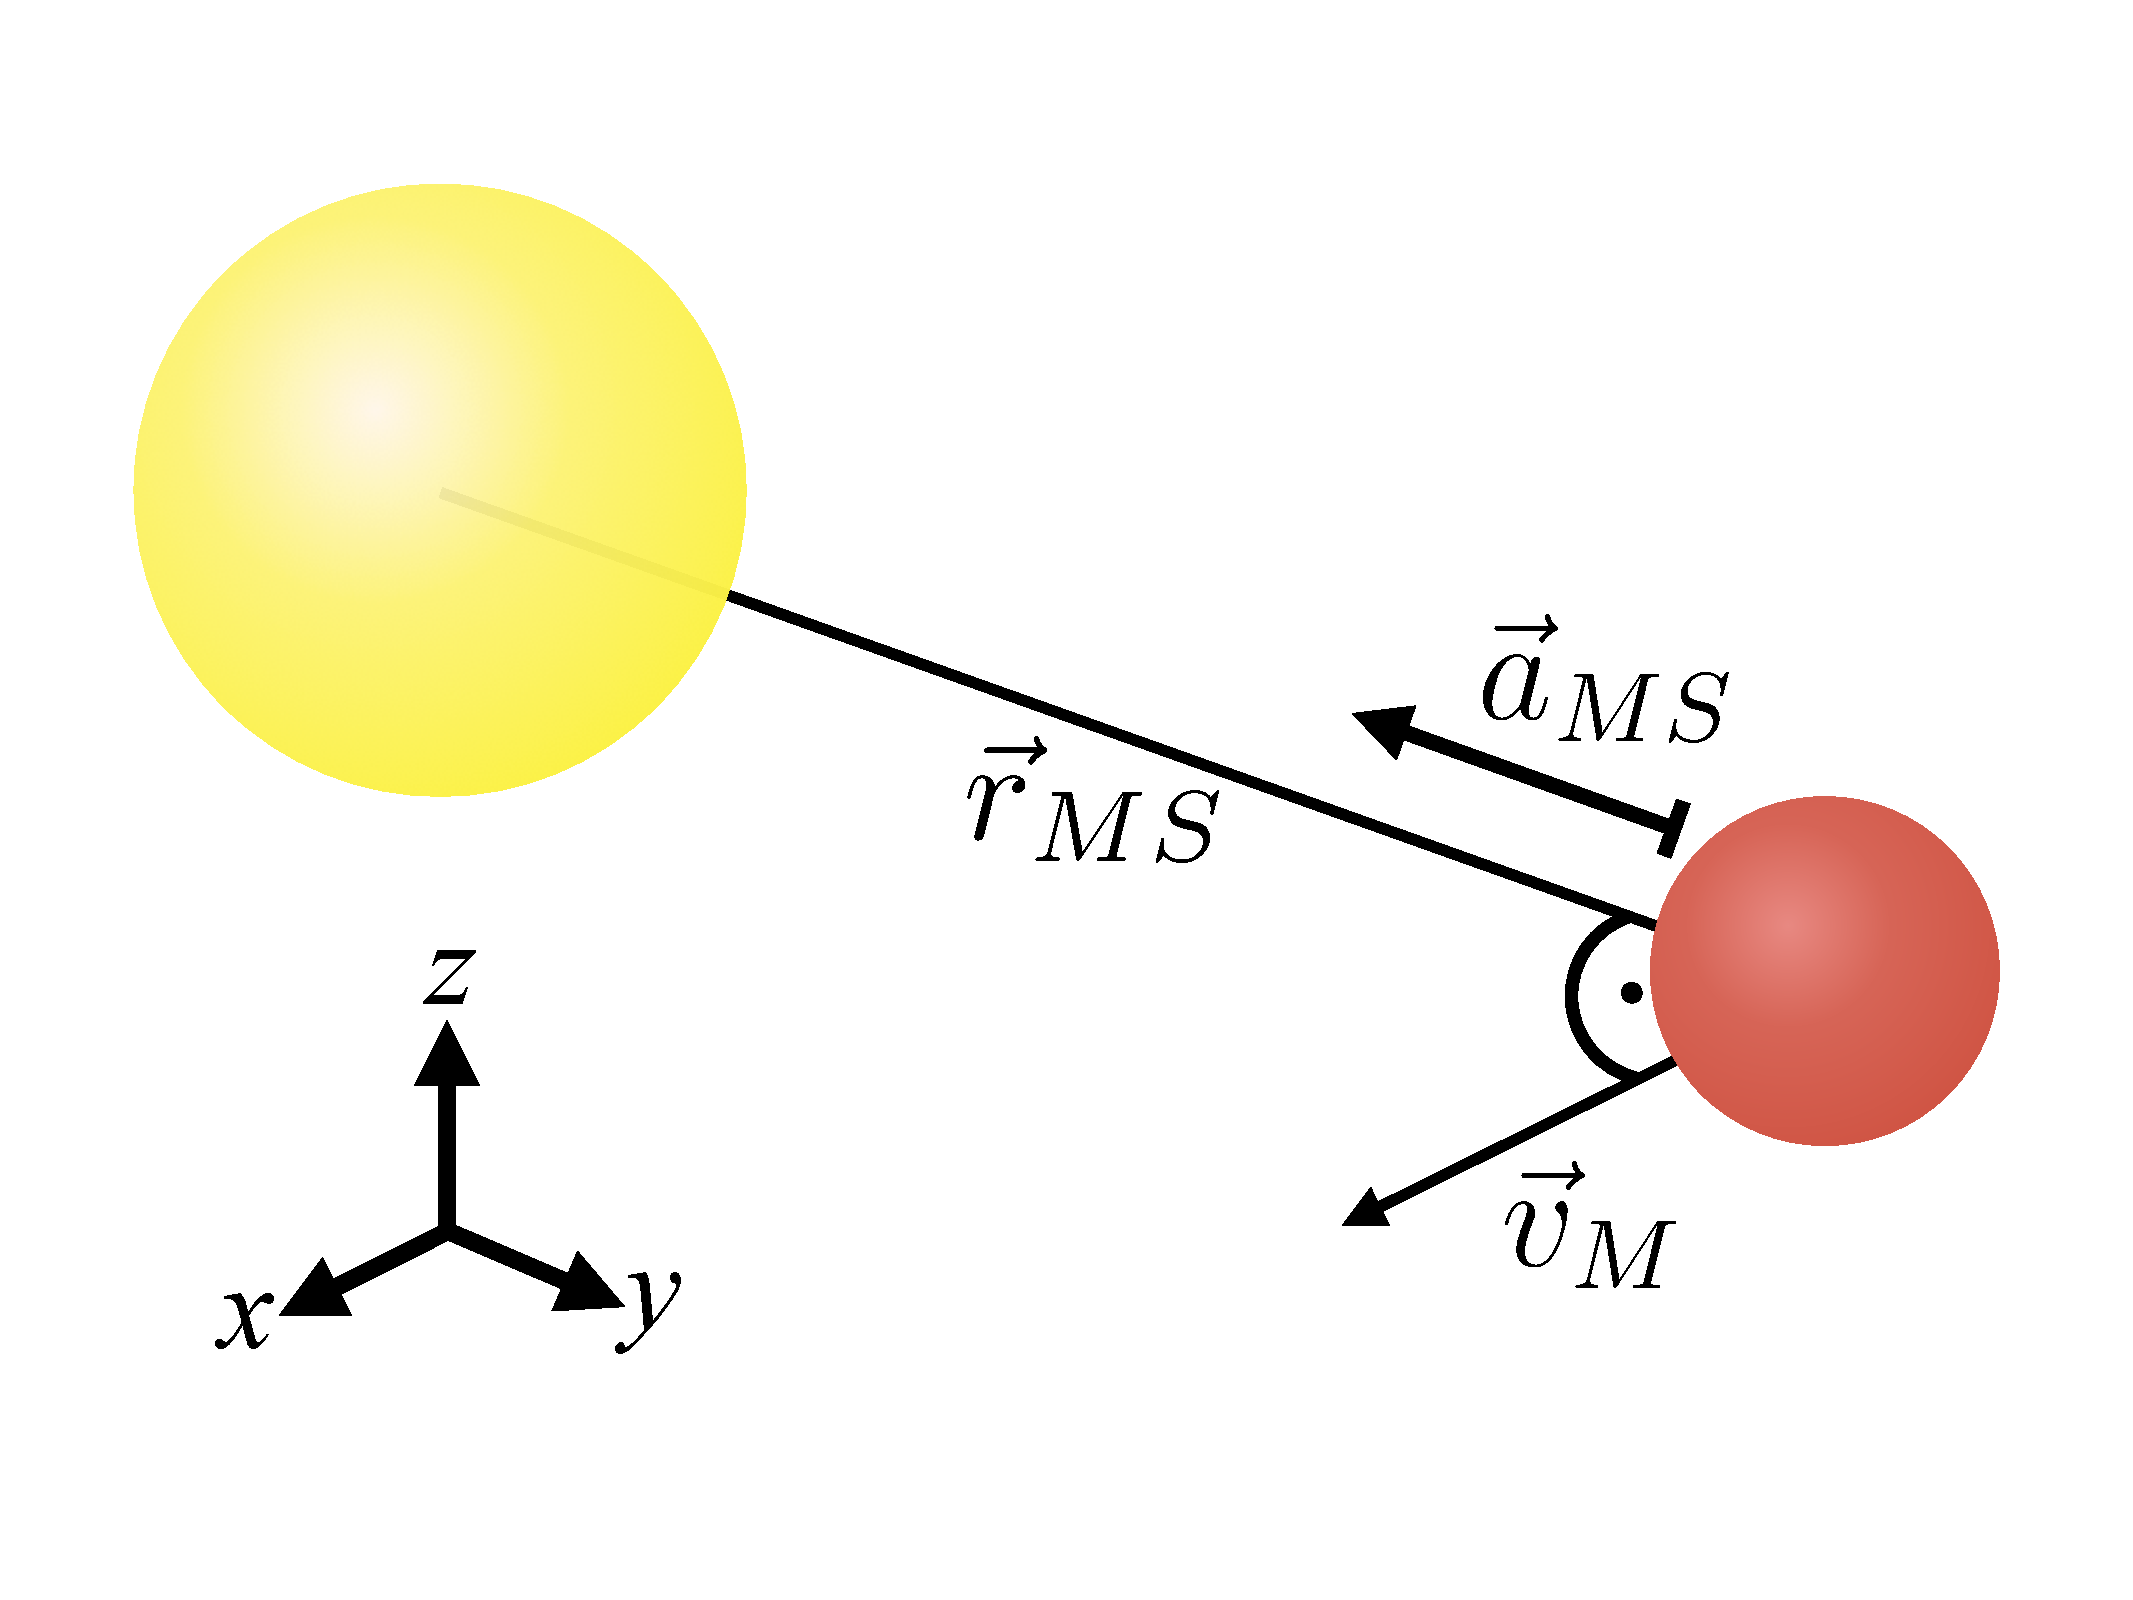
\includegraphics[width=.5\textwidth]{figs/sun_merc.pdf}
	\caption{\label{fig:sun_merc}%
		Sun mercury system with relevant vectors.
		Because mercury is at its perihelion, its velocity is perpendicular to its direct connection vector with the sun.%
	}
\end{figure}
%

In \python{}, this reads
\begin{lstlisting}
# Definition of parameters
rM0 = 4.6    # in units of R0
vM0 = 0.51   # in units of R0/T0
c_a = 1.01   # in units of R0/T0**2
TM  = 88.    # in units of T0
rS  = 3.e-7  # in units of R0
\end{lstlisting}
So far we only fixed the length of the vectors.
Next, we set up the initial directions, which will describe the motion in the two-dimensional plane.  We will build on the existing \python{} module \texttt{VPython}, which provides an implementation for treating vectors as well as their visualization.
The first object of interest is a \texttt{vector}, which takes three-dimensional coordinates as its input.
Because of our choice of initial conditions (we picked the initial vectors in the perihelion), the velocity of mercury is perpendicular to the vector which connects mercury and sun (see figure \ref{fig:sun_merc}):
\begin{lstlisting}
# Import the class vector from vpythons module visual
from vpython import vector
# Initialize distance and velocity vectors
vec_rM0 = vector(0, rM0, 0)
vec_vM0 = vector(vM0, 0, 0)
\end{lstlisting}
According to Eq.~(\ref{eq:newton}), the force which acts on mercury changes the velocity of mercury which eventually changes the position.
However, we first need to fix the time step $\Delta t$ and use the estimate of Eq.~(\ref{eq:check}) as a guidance
\begin{lstlisting}
# Definition of the time step
dt = 2 * vM0 / c_a / 20
\end{lstlisting}
Here the factor $1/20$ makes sure that $\Delta t$ is indeed consistent with Eq.~(\ref{eq:check}).
Now we are in the position to calculate location and velocity of the planet at $t_0+\Delta t$ using the following equations\footnote{%
	Note, that there are different notions for numerically integrating differential equations with different accuracys.
	Thus, the ordering and exact equations for updating $a_{MS}$, $v_M$ and $r_M$ are not unique, but all correct prescriptions lead to the same result for sufficiently small $\Delta t$.
	For this particular problem, the following definition is in good balance between numerically stable and inexpensive to compute.
}%
\begin{lstlisting}
# Compute the strength of the acceleration
aMS = c_a * ( 1 + alpha * rS / vec_rM_old.mag  ) / vec_rM_old.mag**2
# Multiply by the direction
vec_aMS = - aMS * ( vec_rM_old / vec_rM_old.mag )
# Update velocity vector
vec_vM_new = vec_vM_old + vec_aMS * dt
# Update position vector
vec_rM_new = vec_rM_old + vec_vM_new * dt
\end{lstlisting}
Note basic vector operations are already implemented in the predefined \texttt{vector} class.
The difference and sum of two vectors, or the scalar vector multiplication return vectors themselves.
Also the magnitude of a vector --- \texttt{vector.mag} --- is a property of the vector and can be easily extracted.

It is handy to use \texttt{Python}s \texttt{function}s to embed repeating structures ("DRY" --- Don't Repeat Yourself)
\begin{lstlisting}
# Define the coordinate and velocity update function
def evolve_mercury(vec_rM_old, vec_vM_old, alpha):
	# Compute the strength of the acceleration
	aMS = c_a * ( 1 + alpha * rS / vec_rM_old.mag  ) / vec_rM_old.mag**2
	# Multiply by the direction
	vec_aMS = - aMS * ( vec_rM_old / vec_rM_old.mag )
	# Update velocity vector
	vec_vM_new = vec_vM_old + vec_aMS * dt
	# Update position vector
	return vec_rM_new, vec_vM_new

# Call the function
vec_rM_new, vec_vM_new = evolve_mercury(vec_rM_old, vec_vM_old)
\end{lstlisting}
\python{}s syntax enforces a clean programming style: it is necessary that the body of the function is indented (by an arbitrary but consistent amount of \texttt{space}s or \texttt{tab}s) relative to the definition statement of the function.
Furthermore, \python{} is an Interpreter language.
Each line of the code is executed when the Interpreter passes it.
For this reason, all the variables defined before the function are global and thus known to the function.
The variables within the function (e.g. \texttt{aMS}, \texttt{vec\_aMS}, $\dots$) are local and do not exist beyond the scope of the function.

Finally, we can describe the evolution by a \texttt{while}-loop
\begin{lstlisting}%[float,floatplacement=H]
t     = 0
alpha = 0
# Execute the loop as long as t < 2*TM
while t < 2*TM:
	vec_rM, vec_vM = evolve_mercury(vec_rM, vec_vM, alpha)
	t = t + dt
\end{lstlisting}
where for the start we set the parameter $\alpha=0$ in order first study the properties of the pure 
$1/r^2$ force.
Note the required indent of the loop structure similar to the indent of a function.
In each iteration of the \texttt{while}-loop, the previous distance and velocity are used to compute the new values --- which directly overwrites the previous values and thus enter the next iteration.
The total runtime \texttt{2*TM} is the amount of "virtual" days the simulations should run.
To describe at least one full orbital period, this time needs to be larger than $T_M$.
With the previous choice for \texttt{dt}, this corresponds to roughly $N_T \approx 2 \cdot 10^3$ evolution steps.
Note that the exact time it takes for mercury complete a full revolution depends on the initial coordinates and velocities as well as the accuracy of the computation.
One might encourage students to analyze this in the beginning.

%------------------------------------------
\subsection{Visualizing the Motion with VPython}
%------------------------------------------
To start the visualization one has to \texttt{import} further objects from the \texttt{VPython} module.
Additional to the vector class, one has to include
\begin{lstlisting}
from vpython import vector, sphere, color, curve, rate
\end{lstlisting}
The class sphere will represent mercury and the sun in the simulation
\begin{lstlisting}
# define the initial coordinates; M = mercury, S = sun
M = sphere(pos=vec_rM0,       radius=0.5,  color=color.red   )
S = sphere(pos=vector(0,0,0), radius=1.5,  color=color.yellow)
# and the initial velocities
M.velocity = vec_vM0
S.velocity = vector(0,0,0)
# add a visible trajectory to mercury
M.trajectory = curve(color=color.white)
\end{lstlisting}
We have placed the sun in the origin of our coordinate system and choose non-realistic radii sizes for visualization purposes.

Last but not least, instead of updating the object-unrelated vectors in the while loop, we update the object-related vectors which will eventually be drawn
\begin{lstlisting}
t     = 0
alpha = 0
# update the objects
while t < 2*TM:
	# set the frame rate (you can choose a higher rate to accelerate the program)
	rate(100)
	# update the drawn trajectory with the current position
	M.trajectory.append(pos=M.pos)
	# update the velocity and position
	M.pos , M.velocity = evolve_mercury(M.pos , M.velocity , alpha)
	# update time
	t = t + dt
\end{lstlisting}

If the starting values are chosen as advised in the previous section, then the students should end up with a trajectory as depicted in figure \ref{fig:MercuryOrbit-a0-small}.
At this point one might ask students to vary $\Delta t$ and observe its effects on the orbit [see also figure \ref{fig:MercuryOrbit-a0-small-dt-large}].
To get the perihelion motion, the additional force term described in equation (\ref{eq:newton_art}) has to be "turned on" for $\alpha\neq0$ [figure \ref{fig:MercuryOrbit-a6-small}].
This is a good opportunity to let the students play with the size of $\alpha$ and get a feeling for its impact on the trajectories.
However, it might be advisable to not start out with the correct mercury values but a more excentric trajectory by choosing e.g. $r_{MS}(0)=6R_0$ [figure \ref{fig:MercuryOrbit-a6-big}].
Then the perihelion motion is better visible.
\begin{figure}[htb]
	\centering
	\begin{subfigure}[c]{0.22\textwidth}
		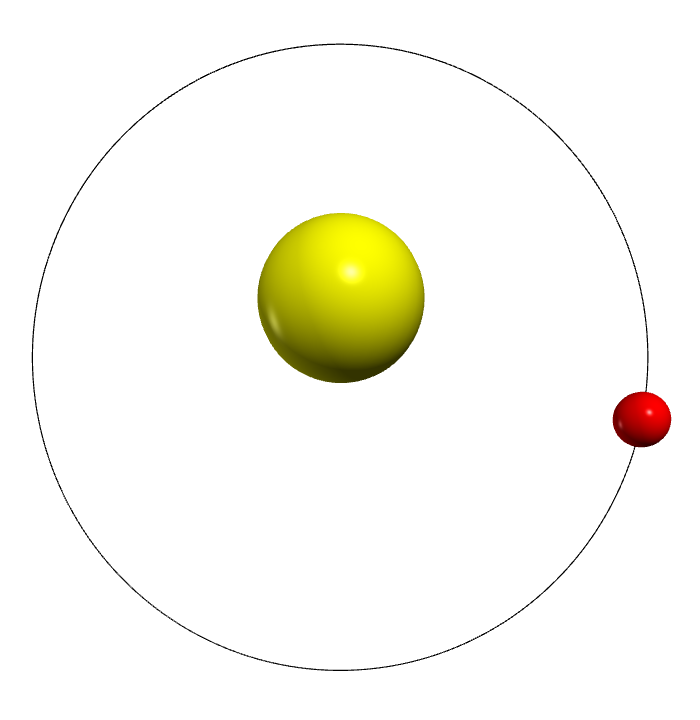
\includegraphics[width=\textwidth]{figs/a0T5dt20.png}
		\caption{\label{fig:MercuryOrbit-a0-small}}
	\end{subfigure}
	~
	\begin{subfigure}[c]{0.22\textwidth}
		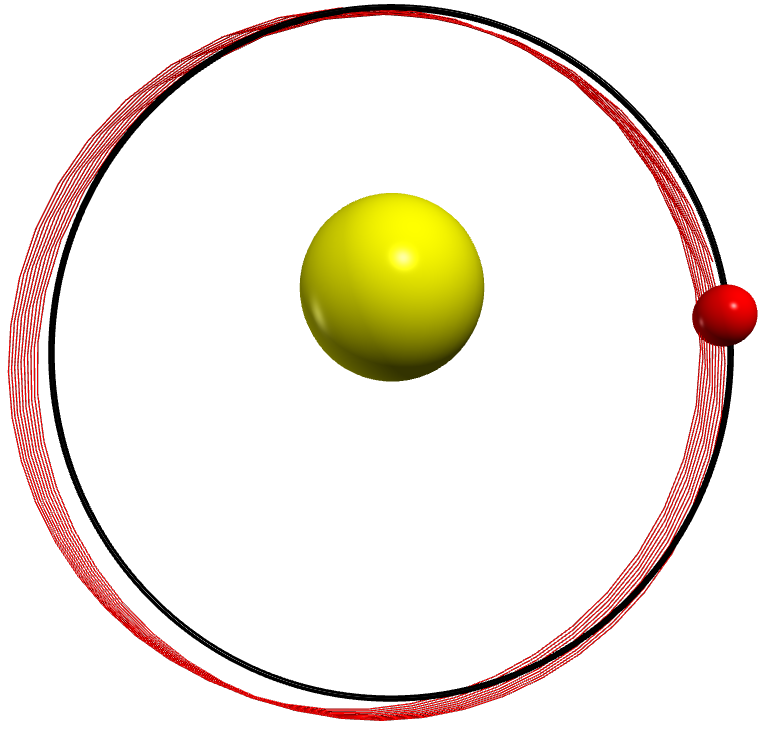
\includegraphics[width=\textwidth]{figs/num-err.png}
		\caption{\label{fig:MercuryOrbit-a0-small-dt-large}}
	\end{subfigure}
	~
	\begin{subfigure}[c]{0.22\textwidth}
		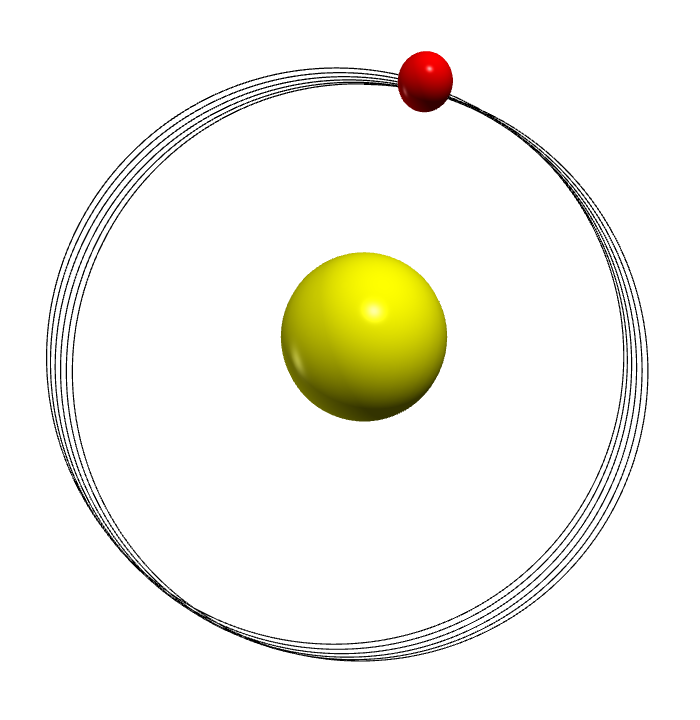
\includegraphics[width=\textwidth]{figs/a6T5dt20.png}
		\caption{\label{fig:MercuryOrbit-a6-small}}
	\end{subfigure}
	~
	\begin{subfigure}[c]{0.22\textwidth}
		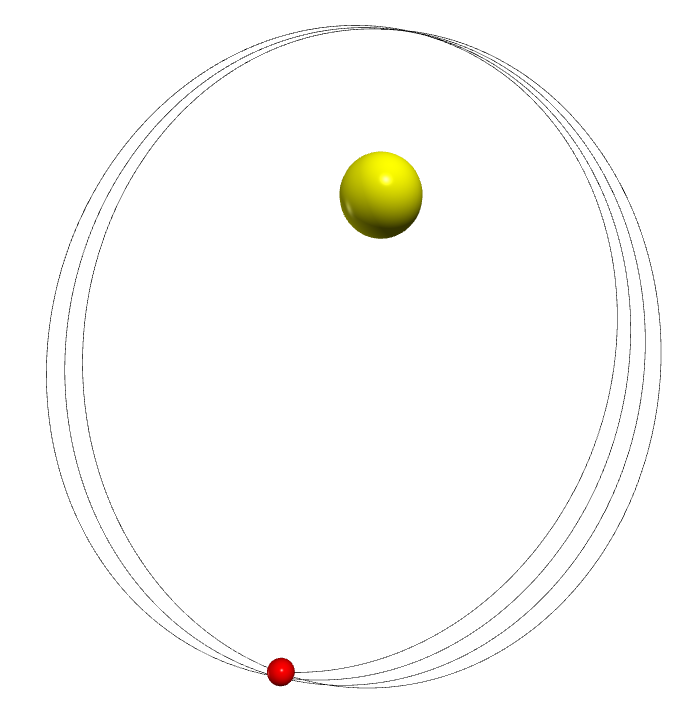
\includegraphics[width=\textwidth]{figs/a6T10dt20.png}
		\caption{\label{fig:MercuryOrbit-a6-big}}
	\end{subfigure}
	\captionsetup{singlelinecheck=off}
	\caption[]{\label{fig:MercuryOrbit}
		Different mercury orbits for:
		\begin{itemize}
		\item[(a)] $\alpha=0$ and $\Delta t = \Delta t_0  / 20$;
		\item[(b)] $\alpha=0$ and $\Delta t = \Delta t_0  \times 2$, where the black line represents the orbit of (a) and the red line is the orbit for the larger time steps;
		\item[(c)] $\alpha=10^{6}$ and $\Delta t = \Delta t_0 / 20$;
		\item[(d)] $\alpha=10^{6}$ and $\Delta t = \Delta t_0 / 20$ but $r_{MS}(0) = 6 R_0$.
		\end{itemize}
		Here, the time steps are defined by $\Delta t_0 \equiv 2 v_{M}(0) / c_a$ and the images are screenshots of the simulation (for modified colors).
		Note that for different starting values of $r_{MS}(0)$, also the numbers of days for a "mercury year" changes.
	}
\end{figure}

%------------------------------------------
\subsection{Extracting the Perihelion Motion}
%------------------------------------------

%\textit{What exactly do we want the students / advise the teachers to do? I think a nice approach would be to let the students implement the code to extract the perihelion motion and make a list of some values of alpha and the corresponding angles. Then discuss, that $\alpha=1$ is the natural size for $\alpha$ and that to extract the value of angle they need to exploit the linear dependence. Finally they can think on whether the value they get is reasonable and the teacher can explain the rest of section? What do you think?}\\

To calculate the expected size of the perihelion motion for a modified gravitational force, the students need to
\begin{itemize}
\item extract multiple positions of the perihelion $\vec r_{MS} ( t_\mathrm{ph}^{(n)} )$ for a fixed value of $\alpha$ and simulations times which covers several orbits;
\item calculate the angle between the perihelions for two successive turns and compute the average angle $\delta \Theta (\alpha)$ over all individually computed angles;
\item repeat the above points for different values of $\alpha$ to confirm the linear dependence of $\delta \Theta (\alpha)$;
\item interpolate $\delta \Theta (\alpha)$ to $\alpha=1$ using that $\delta \Theta (0) = 0$ (modulo numerical errors).
\end{itemize}

There are several ways to find the position of the perihelion.
The easiest one is to look for the point of minimal distance to the sun --- the definition of the perihelion.
This can be done within the $while$-loop.
To find identify a minimal distance to the sun, one has to know the last two positions \texttt{vec\_r\_last} and \texttt{vec\_r\_before\_last} in addition to the current position.
If the length of the \texttt{last} vector is smaller than that of the \texttt{before\_last} vector and smaller than the current vector, one has passed the perihelion and its position is given by \texttt{vec\_r\_last}.
It is useful to save the position of the perihelion in a list \texttt{list\_perih} for a certain number of turns (here e.g. \texttt{max\_turns}=10).
The implementation can be realized as follows\footnote{%
	Note that one stores \code{vec\_r\_last} by making a copy of \code{M.pos}: \code{vec\_r\_last = vector(M.pos)}.
	This is essential because otherwise, if one changes \code{M.pos}, one would automatically change \code{vec\_r\_last} as well.
}
\begin{lstlisting}
# set up vectors
vec_r_last = vec_rM0
turns      = 0
max_turns  = 10
list_perih = list()
# find perihelion for each turn and print it out
while turns < max_turns:
	vec_r_before_last = vec_r_last
	# store position of mercury in a new vector (since we will change M.pos)
	vec_r_last = vector(M.pos)
	#<...update mercury position...>
	# check if at perihelion
	if (vec_r_last.mag < M.pos.mag) and (vec_r_last.mag < vec_r_before_last.mag):
		list_perih.append(vec_r_last)
		turns = turns+1
\end{lstlisting}
To compute the angle between two vectors one uses the following
formula
 \begin{equation}
 	\sphericalangle(\vec{v}_{1},\vec{v}_2) = \mathrm{arccos} \left( \frac{\vec{v}_{1} \cdot \vec{v}_2}{|\vec{v}_{1}|\:|\vec{v}_2|} \right)
	\, .
 \end{equation}
This is readily implemented in \texttt{VPython} via
\begin{lstlisting}
# import function to resolve angle
from vpython import acos, pi, dot
# define function for angle extraction
def angle_between(v1, v2):
	return acos( dot(v1, v2) / (v1.mag * v2.mag) ) * 180. / pi
\end{lstlisting}
To account for the statistical errors (e.g., numerical rounding errors) one can average over a few turns.
Depending on the programming proficiency of the students and time constraints, this can be either done by hand or, e.g., by implementing the following code
\begin{lstlisting}
sum_angle=0.
for n in range(1, max_turns):
	# calculate angle
	sum_angle = sum_angle + angle_between(list_perih[n-1], list_perih[n])
# display the average
print(sum_angle/(max_turns-1.))
\end{lstlisting}

As explained above [and further discussed in chapter \ref{sec:analysis}] the natural value for $\alpha$ would be of the order of $1$.
However, if the students use this value for $\alpha$, they will find that the change in the trajectories is close to invisible and the numerical uncertainty is much larger than the result.
Therefore, to estimate the size of the perihelion motion, it is more advisable to use the fact that there is a linear dependence between $\alpha$ and $\delta \Theta$\footnote{%
	Of course for very large values of $\alpha$ this linear relation will eventually break down.
	We therefore advise to choose $\alpha<7\cdot 10^6$ at which point the perihelion motion exceeds $\delta \Theta=90^{\degree}$.
}.
The students can convince themselves of this fact by plotting the angles $\delta \Theta$ they have extracted from their simulation over $\alpha$.
This can be done either by hand, \python{} (e.g., with \texttt{matplotlib}: \url{https://matplotlib.org}), or using another program like, e.g., Excel.
For instance figure \ref{fig:AlphaAngle} demonstrates such a plot.

\begin{figure}[htb]
	\centering
	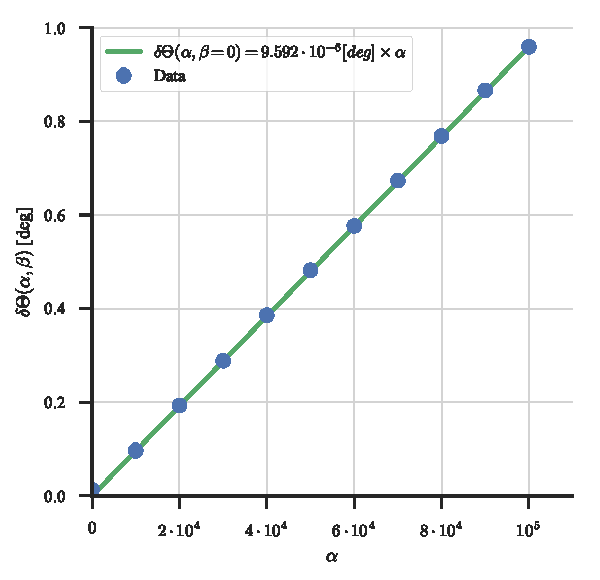
\includegraphics{figs/alpha-angle.pdf}
	\caption{\label{fig:AlphaAngle} Linear relation between $\alpha$ and the perihelion motion $\delta \Theta$ for $\Delta t=2v_M(0)/c_a/100$.}
\end{figure}

To extract the perihelion motion at $\alpha = 1$, we use the fact that $\delta \Theta$ is zero for $\alpha =0$ --- if one could completely eliminate numerical errors.
Considering one result from the numeric simulation, e.g. $\delta\Theta(\alpha = 10^6) \approx 10.0^{\degree}$, the sought-after angle can be calculated by a linear interpolation as
\begin{equation}
	\delta\Theta (\alpha=1) = \frac{10.0^{\degree}}{10^6} = 0.036''
	\, .
\end{equation}
Depending on the knowledge of the students, multiple points and also estimated numerical uncertainties could be used to extract this value by a linear regression.
Note that, when comparing the results of the simulation with the experimental result, one Earth year corresponds to $T_E/T_M \approx 365d/88d\approx 4.15$ mercury years.
Therefore, the perihelion motion per 100 earth years is $0.036''\cdot 415\approx 15''$.
To test whether this is a reasonable result, the students could first follow the dimensional analysis and then compare to the actual value for mercury as outlined above.

%%%%%%%%%%%%%%%%%%%%%%%%%%%%%%%%%%%%%%%%%%%%%%%%%%%%%%%%%%%%%%%%%%%
\section{Tests of stability and error analysis}\label{sec:stability}
%%%%%%%%%%%%%%%%%%%%%%%%%%%%%%%%%%%%%%%%%%%%%%%%%%%%%%%%%%%%%%%%%%%
\todo[inline]{@all: where is this periodic oscillation coming from?}
Physical experiments in general, as do numerical simulations of physics, must always account for possible uncertainties.
It is important for the students to recognize this fact and to understand, that the cause of the uncertainties lies, e.g., in the finite time steps.
The students should therefore explore the source and size of the errors arising in this simulation at least qualitatively.

Consider figure \ref{fcc3}, where the angle of the perihelion growth $\delta \Theta$ is shown for the first $10$ turns for different choices of $\Delta t$ (colors) and $\alpha$ (columns).
As expected, the correlation between the number of turns and $\delta\Theta$, for sufficiently small time-steps $\Delta t$, is constant on average and the values depend solely on $\alpha$.
However, there is an offset between the lines for different $\Delta t$.
The reason is, due to the uncertainties in the simulation, the starting position does not coincide with the first perihelion as one might expect.
This does not generate a problem for the procedure described in the previous section since the starting position is not considered. Still, it is helpful to be aware of this fact.
One can see nicely in figure \ref{fcc3} that the oscillations of the perihelion motion increases for growing time steps. 

\begin{figure}[htb]
	\centering
	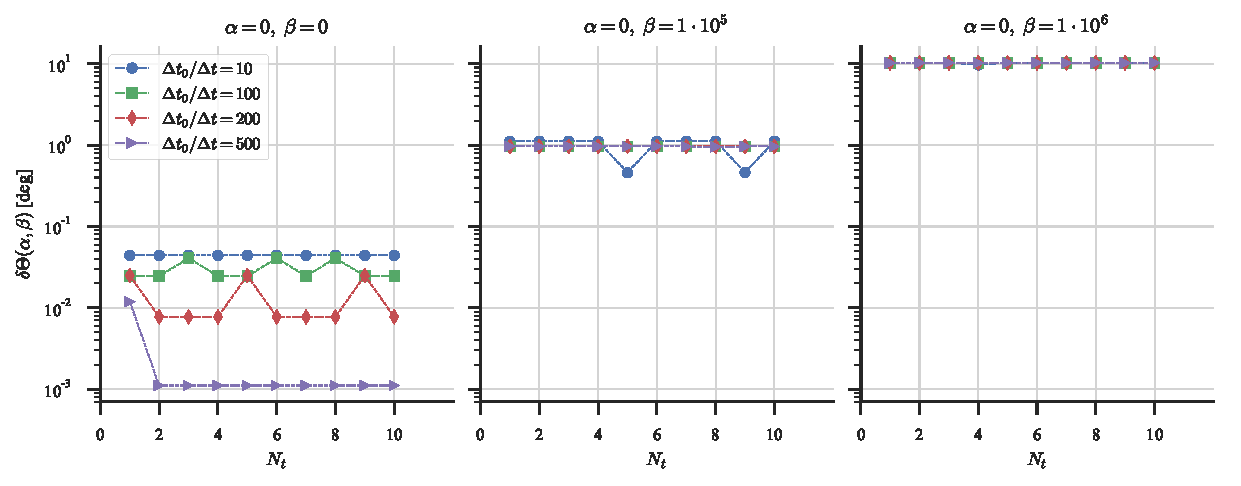
\includegraphics[width=.99\textwidth]{figs/angular-variaton.pdf}
	\caption{\label{fcc3}Precession growth of perihelion $\delta\Theta$ in degrees depending on the number of turns $N_t$ for different time steps $\Delta t$ (color) and different values for $\alpha$ (columns).
	Here, $\Delta t_0 \equiv 2 v_M(0)/c_a$.
	One should pay special attention to the oscillations within the growth for relatively large time steps.
}
\end{figure}

To point the students to this problem, they can be asked to increase their time steps significantly and observe the effect on the trajectories.
For this study, it is advantageous to set $\alpha =0$, since in this case the trajectories should be closed and therefore deviations from the ideal case can be spotted easily.
In figure \ref{fig:MercuryOrbit-a0-small-dt-large} the mercury trajectory for $\Delta t=2 v_M(0) / c_a \times 2$ is shown.
One can clearly see the failure of the simulation to reproduce the physical trajectory.
From examples like this it should be apparent that the time steps influence the accuracy of the simulation.
One could quantify the deviation of $\delta\Theta$ from zero and use this to estimate the numerical systematic uncertainty for a given time step $\Delta t$.
Only in the limit $\Delta t \rightarrow 0$ would the simulation perfectly reproduce the actual trajectory.


%%%%%%%%%%%%%%%%%%%%%%%%%%%%%%%%%%%%%%%%%%%%%%%%%%%%%%%%%%%%%%%%%%%
\section{Dimensional analysis}\label{sec:analysis}
%%%%%%%%%%%%%%%%%%%%%%%%%%%%%%%%%%%%%%%%%%%%%%%%%%%%%%%%%%%%%%%%%%%

Dimensional analysis is not only a tool that allows one to cross check if the results of some simulation is of the right order of magnitude, it is also very helpful to identify unusual dynamics in some system.
Especially the latter aspect should become clear from the discussion in this section.

The idea of dimensional analysis is that in a system that can be controlled by expanding the relevant quantities (like the force) in some small parameter(s), the coefficients in the expansion should turn out to be of order unity (that means anything between about 0.1 and 10 is fine - but 0.01 or 100 is irritating) --- parameters in line with this are called "natural".
Applied to the problem at hand given by Eq.~(\ref{eq:newton}) this statement implies that from naturalness one would expect that the parameter $\alpha$ is of order 1 when one uses for $r$ the average distance Mercury-sun, namely $\bar r=6\times 10^7$ km.
From this one estimates for the expected angular shift per orbit
\begin{equation}
\delta \Theta \simeq 2\pi\left(\frac{r_S}{\bar r}\right) = (\pi \times 10^{-7}) \ \mbox{rad} = (2\times 10^{-5})^o = (7\times 10^{-2}) ^{''} \ ,
\end{equation}
which leads to a shift of about $30^{''}$ in 100 earth years to be compared to the empirical value of $43^{''}$.
Thus indeed the amount of perihelion motion of Mercury is in line with expectations, $if$ --- and this is an important "if" --- the Newtonian dynamics is simply the leading term of some more general underlying theory.
In particular, no new scales enter in the correction terms.

Thanks to Einstein we indeed know that the conclusion formulated above is correct --- the more general underlying theory is General Relativity and indeed Einstein was able to quantitatively explain the perihelion motion of Mercury from his equations. 
On the other hand had we found a dramatic deviation of $\alpha$ from unity one would have concluded that there is probably some other dynamics going on that drives this difference.

Indeed, we now several of those hierarchy problems in modern physics: e.g., the so called QCD $\Theta$ term, expected to be of natural size, is at present known to be at most $10^{-10}$.
This smallness, called the strong CP problem, is so irritating that physicists like S. Weinberg even proposed that there must exist an additional particle, the axion, whose interactions are in charge of pushing $\Theta$ even to zero and there are now intense searches for this axion going on various labs.



%%%%%%%%%%%%%%%%%%%%%%%%%%%%%%%%%%%%%%%%%%%%%%%%%%%%%%%%%%%%%%%%%%%
\section{Tasks}\label{sec:tasks}
%%%%%%%%%%%%%%%%%%%%%%%%%%%%%%%%%%%%%%%%%%%%%%%%%%%%%%%%%%%%%%%%%%%
\todo{@IH: this could be a little bit more verbose. Maybe include in section below.}
Ideas for questions:
\begin{itemize}
	\item Mass and motion of sun
	\item Estimate \texttt{dt} and also \texttt{T} in order to cover roughly two "mercury years".
	\item What does happen when you change those units?
	\item Compare values to the values in \cite{}.  Where does the difference come from?
	\item Start with $\alpha=0$. What do you observe?
\end{itemize}



%%%%%%%%%%%%%%%%%%%%%%%%%%%%%%%%%%%%%%%%%%%%%%%%%%%%%%%%%%%%%%%%%%%
\section{Possible extensions}\label{sec:extensions}
%%%%%%%%%%%%%%%%%%%%%%%%%%%%%%%%%%%%%%%%%%%%%%%%%%%%%%%%%%%%%%%%%%%

\begin{itemize}

\item \textbf{Explore Problem autonomously}

In chapter \ref{sec:Numerical Implementation} we suggested to present the material by using a template as well as a step by step instruction to guide the students through the problem solution.
These instructions can be cut down or left out depending on available time and numerical/computational versatility of the students.
This could be achieved by the following changes or additions to the concept presented in chapter \ref{sec:Numerical Implementation}.

\begin{itemize}
\item \textbf{Build code from scratch}

Instead of providing the template to the students, they could build the program from scratch.
Of course, this requires some basic knowledge in \texttt{VPython}, as they could acquire for example by working through a ball in the box example\cite{}\todo{@IH: cite ball in the box} or the like.
Also, they could independently research the problem relevant parameters.
\item \textbf{Why can we work in one plane?}

In the code the third coordinate ($z$) is never used.
On the first glance, this might seem like a simplification.
The students could work out on their own, why this does not imply any loss of generality.
\item \textbf{What is the impact of the different parameters?}

Especially if the needed parameters are not specified beforehand, the students might have to experiment a bit, before getting the correct trajectories.
But even if they are given, it might be beneficial to encourage the students to play with a few parameters, like the masses or the starting velocities, and observe their impact on the trajectories.
This way the students get a better feeling for the physics involved.
\end{itemize}

\item \textbf{Optimizing performance}

Simulations always involve a balance between the time needed for the calculations and the demanded accuracy for the results.
Even though this is a rather simple example, it contains some opportunities to make these concepts accessible to the students.

\begin{itemize}
\item \textbf{Consider error due to finite time steps}

To make the students realize that the finite time steps lead to inaccuracies in the trajectories, one can propose to test this by increasing the size of the time steps.
This is best done in a program with unmodified gravitational force ($\alpha=0$), since in this case the trajectories are closed ellipses and numerical errors are most prominently visible in form of deviations from a bounded orbit.
If the students choose the time steps big enough, they should witness big deviations.
This exercise stresses the point, that by choosing increasingly smaller time steps, deviations from the physical trajectories can be reduced.
\item \textbf{Measure calculation time}

However in practice there is a limit to decreasing the time steps, because the time needed for the calculation grows simultaneously.
By including \texttt{import time}
\begin{lstlisting}
start_time = time.time()
main()
print("--- %s seconds ---" % (time.time() - start_time))
\end{lstlisting}
the students can measure the time needed by their program.
By varying $\Delta t$ they can validate, that there is indeed approximately an anti-proportional dependence.
(Note: This only works if the time in the loop is increased by $\Delta t$, so $t=t+\Delta t$.)
\item \textbf{Verlet integration}

Of course by optimizing the code, an improvement in accuracy can be achieved without changing $\Delta t$.
The simplest way to demonstrate this might be given by the implementation of the Verlet\cite{}\todo{@IH: cite Verlet} integration instead of using the simple Euler method.
\end{itemize}

\item \textbf{Extended Problems}

\begin{itemize}
\item \textbf{Non-stationary sun}

It might be interesting to abandon the simplification of a stationary sun, as it nicely illustrates Newton's third law.
Here it might also be advisable to reduce the mass of the sun to have a more visible result.

\item \textbf{Three-body problem}

Ambitious students could even include further planets and see how the different planets interact.
This is especially interesting, when discussing the perihelion motion of mercury, as it is mainly due to the influence of the other planets.
Only a smaller part is due to general relativity.

\end{itemize}

\end{itemize}

%%%%%%%%%%%%%%%%%%%%%%%%%%%%%%%%%%%%%%%%%%%%%%%%%%%%%%%%%%%%%%%%%%%
\appendix
%%%%%%%%%%%%%%%%%%%%%%%%%%%%%%%%%%%%%%%%%%%%%%%%%%%%%%%%%%%%%%%%%%%



%%%%%%%%%%%%%%%%%%%%%%%%%%%%%%%%%%%%%%%%%%%%%%%%%%%%%%%%%%%%%%%%%%%
\section*{Acknowledgments}
%%%%%%%%%%%%%%%%%%%%%%%%%%%%%%%%%%%%%%%%%%%%%%%%%%%%%%%%%%%%%%%%%%%
\todo{@all: Acknowledgments}
Here they come



%%%%%%%%%%%%%%%%%%%%%%%%%%%%%%%%%%%%%%%%%%%%%%%%%%%%%%%%%%%%%%%%%%%
\section{Instructions to install VPython}\label{appendix:python}
%%%%%%%%%%%%%%%%%%%%%%%%%%%%%%%%%%%%%%%%%%%%%%%%%%%%%%%%%%%%%%%%%%%
In short, to run the above scripts, one needs to install \python{} and \vpython{}.
We recommend the newest \vpython{} version 7 or higher which best runs with the \python{} versions of 3.5 or higher.
It is also possible to use \python{} 2.7 or higher, but the 3.x versions have better \vpython{} support.

For the advanced users, one simply has to update \python{} to these versions and install \vpython{} via the package manager of choice, e.g, \texttt{pip} [see also \url{http://vpython.org}].

Below, we provide detailed descriptions how to install these versions of \python{} and \vpython{} for different operating systems.
Independent of the operating systems, one has to execute the following steps:
\begin{enumerate}
	\item install and update \python{} (at best 3.x, x$\geq5$);
	\item install and update a \python{} package manager;
	\item install \vpython{} and dependencies.
\end{enumerate}

%%%%%%%%%%%%%%%%%%%%%%%%%%%%%%%%%%%%%%%%%%%%%%%%%%%%%%%%%%%%%%%%%%%
\subsection{Linux based systems (including macOS)}\label{appendix:python-max}
%%%%%%%%%%%%%%%%%%%%%%%%%%%%%%%%%%%%%%%%%%%%%%%%%%%%%%%%%%%%%%%%%%%
All Linux based system come with an installation of \python{}.
Thus, if not already at the newest version, one just has to update existing installations.
This is best done by using a distribution manager.
Native to Linux based systems is for example \texttt{dpkg} and \texttt{apt-get}, or \texttt{homebrew} and \texttt{MacPorts} for macOS.
While \texttt{dpkg} and \texttt{apt-get} usually come with the linux installations, macOS user must install such distribution managers at first.
For this we refer to \url{https://www.macports.org/install.php} or \url{https://docs.brew.sh/Installation.html}.

As the start one should open a terminal/console (bash).
Depending on the installation, one usually needs superuser rights in order to update \python{}.
Therefore one has to prepend \code{sudo} to the following commands and confirm them by entering the superuser password.
The installations using a distribution manager are save and tested by the vast community.
In the following, the successive order of commands to update \python{} is presented for \texttt{apt-get} (Linux) and \texttt{MacPorts} (macOS), but are most similar for other distribution managers.
\begin{table}[h!]
\centering
\footnotesize
\begin{tabular}{l || l | l}
	& \texttt{apt-get} & \texttt{MacPorts} \\\hline
	1. Update the distribution manager & \code{sudo apt-get update} & \code{sudo port selfupdate} \\
	2. Install \& update \python{} & \code{sudo apt-get install python3} & \code{sudo port install python36} \\
	3. Installing \python{} package manager & \code{sudo apt-get install python3-pip} & \code{sudo port install py36-pip}
\end{tabular}
\normalsize
\end{table}

Depending on the previously installed packages, this command might install further dependencies automatically (after confirmation).
One should test if the installation was successful by typing \code{python3 --version} or \code{python3.6 --version} (depending on the installation name) which prints out the version of the \python{} installation (and should be larger than 3.5).
Next one must update the package manager to get the newest versions of \python{} packages.
This is done by running
\begin{table}[h!]
\centering
\footnotesize
\begin{tabular}{l || l | l}
	& \texttt{apt-get} & \texttt{MacPorts} \\\hline
	4. Update \code{pip} & \code{pip3 install --upgrade --user pip wheel} & \code{pip-3.6 install --upgrade --user pip wheel} \\
\end{tabular}
\normalsize
\end{table}\\
Note that this just upgrades the packages for the current user.
If one wants the systemwide installation, one again has to prepend \code{sudo} and can ignore the \code{--user} flag (\code{sudo pip3 install --upgrade pip wheel}).
Furthermore, depending on the installed version of \code{pip}, it could have a different name.
This is best figured out by typing \code{pip} and pressing \texttt{tab}.

Finally, one can install \vpython{} by running
\begin{table}[h!]
\centering
\footnotesize
\begin{tabular}{l || l | l}
	& \texttt{apt-get} & \texttt{MacPorts} \\\hline
	5. Install \vpython{} & \code{pip3 install --user vpython} & \code{pip-3.6 install --user vpython} \\
\end{tabular}
\normalsize
\end{table}

At this point, everything is installed and one can start the simulation.
To test the \vpython{} installation one should run \code{python3} or \code{python3.6}, which starts a \python{} console.
Next, one shall run \code{from vpython import *}, which loads the \vpython{} package and opens the default browser.
Running \code{box()} should generate a white box in the browser window, which can be rotated using the mouse.
The program is quit by running \code{quit()} or pressing \texttt{Ctrl-c}.

In general, there are multiple ways to run \python{} scripts.
For the sake of this paper, we suggest two scenarios.
\begin{enumerate}
\item The first scenario to run \python{} scripts is that one writes and saves a \python{} file, e.g., \texttt{test.py}, which can be edited using any text editor of choice.
	To run the \python{} script one must navigate the terminal to the containing folder using the \code{cd} (and \code{ls}) command.
	While \code{ls} prints out the folders and files in the current directory, \code{cd} changes the directory.
	The command \code{cd} either takes relative paths (directories which are in the current directory), e.g., \code{cd folder}, or absolute paths beginning with a \code{/}, e.g., \code{cd /Users/name/Desktop/}.
	Once one has navigated to folder which contains the \python{} file --- e.g., the file name is listed when typing \code{ls} --- than one can type \code{python3 test.py} or \code{python3.6 test.py} to execute the script.
	Again, this script can be ended (if it does not end automatically) by pressing \texttt{Ctrl-c}.
\item The second scenario to run \python{} scripts is given by the interactive \texttt{ipython} or \texttt{jupyter} notebooks.
	This feature is automatically installed when installing the newest version of \vpython{}.
	To start an interactive session, one has to run \code{jupyter notebook} (or equivalent, depending on the installation name. Again, this can be figured out by typing \code{jupyter} and pressing \texttt{tab}).
	This will print a link (containing the name \texttt{localhost}) and open the browser at the link-address.
	Within this browser window, one can freely navigate to the directory of choice and create interactive \python{} and \vpython{} sessions by clicking on existing files or creating new ones (upper right button \texttt{new}$\rightarrow$\vpython{}).
\end{enumerate}
We provide example files for both scenarios.\todo{@arXiv: online link}

%%%%%%%%%%%%%%%%%%%%%%%%%%%%%%%%%%%%%%%%%%%%%%%%%%%%%%%%%%%%%%%%%%%
\subsection{Windows}\label{appendix:python-windows}
%%%%%%%%%%%%%%%%%%%%%%%%%%%%%%%%%%%%%%%%%%%%%%%%%%%%%%%%%%%%%%%%%%%

As the first step, one must install \python{}, again there are several possibilities but we suggest \texttt{Anaconda} for an intuitive installation.
Following the link \url{https://conda.io/docs/user-guide/install/download.html}, one has two possible (free) options, \texttt{Anaconda} and \texttt{Miniconda}.
Both are equally sufficient.
One can install further updates after the initial installation.
In the case of \texttt{Miniconda} (\url{https://conda.io/miniconda.html}) one shall download the newest \python{} 3.x (x $\geq5$) installer for windows and the right system type (32-bit or 64-bit).
The system type can be found by pressing \texttt{Windows+I}, navigating to \texttt{System}$\rightarrow$\texttt{About} and looking at the \texttt{System type} entry.

Installing one of the two executables creates a new \texttt{Windows} application called \texttt{Anaconda Prompt}.
Starting this application opens a terminal which will be used to install the required \python{} packages.
At first, one should test if the \texttt{Anaconda} installation was successful by running the command \code{conda list}.
This command should print a list of already installed packages.
Also one should run \code{conda update conda} to make sure one has the most recent installation.

To install \vpython{} one simply has to run \code{conda install -c vpython vpython}.
The additional flag \code{-c vpython} tells \texttt{Anaconda} the "channel" where to look for the \vpython{} package.
Running this command prints out a list of dependencies which will be automatically installed in order for \vpython{} to work --- this must be confirmed.

In principle this is already sufficient to run \vpython{} scripts.
One could furthermore install \texttt{Anaconda}s native navigator \texttt{anaconda-navigator} by running \code{conda install anaconda-navigator}.
This will install another application, \texttt{Anaconda Navigator}, which can be run from the Desktop and makes it easier to program in \python{}.

Again there are several possibilities to run \python{} files on \texttt{Windows}.
\begin{itemize}
	\item One could create a file \texttt{test.py}, edit it with the editor of choice and specify that this file should be opened with \texttt{Python3}.
		To do so, \texttt{right click} on  the file, select \texttt{open with} and locate the \texttt{Anaconda Python3} installation.
		Programs can be closed by closing the running window.
	\item One can run \code{python3} in the \texttt{Anaconda Prompt} application to start an interactive session.
		Programs can be closed by closing the running window.
	\item Start the \texttt{Anaconda Navigator} application, open an interactive \texttt{qtconsole} and program within the newly opened terminal.
		Programs can be closed by closing the running window.
	\item Start the \texttt{Anaconda Navigator} application and click on the \texttt{jupyter notebook} button.
		This opens an interactive \python{} session in the default web-browser.
		Here, one can open existing notebooks or create new files (upper right button \texttt{new}$\rightarrow$\vpython{}).
\end{itemize}

To start and test the \vpython{} installation one should pick any out of these options and execute the code
\begin{lstlisting}
from vpython import *
box()
\end{lstlisting}
Running this code should open the default browser and render a white box on black background.
Using the mouse (right click and drag), one should be able to rotate the box.
It was found that the \texttt{Internet Explorer} is not able to properly render the animation.
Here we suggest to use the \texttt{Firefox} web-browser as the default choice.

Once this test case works, one can start to test the mercury orbit simulation.
We provide example files for both \texttt{juypter notebooks} and regular \python{} files.

\todo{@arXiv: online link}



%%%%%%%%%%%%%%%%%%%%%%%%%%%%%%%%%%%%%%%%%%%%%%%%%%%%%%%%%%%%%%%%%%%
\clearpage
\section{The code}\label{sec:code}
%%%%%%%%%%%%%%%%%%%%%%%%%%%%%%%%%%%%%%%%%%%%%%%%%%%%%%%%%%%%%%%%%%%
Below we provide an example script on how to program the visualization of the mercury orbit in \vpython{}.
\lstinputlisting[language=Python]{mercury_orbit_base.py}
Further examples and template files can be found online\cite{}.\todo[inline]{@arXiv: online link}




%%%%%%%%%%%%%%%%%%%%%%%%%%%%%%%%%%%%%%%%%%%%%%%%%%%%%%%%%%%%%%%%%%%
% Bib
%%%%%%%%%%%%%%%%%%%%%%%%%%%%%%%%%%%%%%%%%%%%%%%%%%%%%%%%%%%%%%%%%%%
%\bibliographystyle{alphadin}
%\bibliography{MercuryNumerical}
%%%%%%%%%%%%%%%%%%%%%%%%%%%%%%%%%%%%%%%%%%%%%%%%%%%%%%%%%%%%%%%%%%%

\end{document}